\chapter{File System}
\newpage
\section{Introduzione}
I computer possono utilizzare diversi media per registrare in
modo permanente le informazioni
\textit{esempi: dischi rigidi, floppy, nastri, dischi ottici}

Ognuno di questi media ha caratteristiche fisiche diverse
Compito del \textbf{file system} è quello di astrarre la complessità di utilizzo dei diversi media proponendo una interfaccia per i sistemi di memorizzazione: comune, efficiente
conveniente da usare.

Dal punto di vista dell’utente, un file system è composto da
due elementi:
\begin{itemize}
    \item \textbf{file}: unità logica di memorizzazione.
    \item \textbf{directory}: servono per organizzare e fornire informazioni sui file che compongono un file system.
\end{itemize}

Il concetto di file è l'entità atomica di assegnazione/gestione della memoria secondaria,  è una collezione di informazioni correlate che fornisce una vista logica uniforme ad informazioni correlate.

\subsubsection{Attributi dei file}
\paragraph{}
\textbf{Nome}: stringa di caratteri che permette agli utenti ed al sistema operativo di identificare un particolare file nel file system, alcuni sistemi differenziano fra caratteri maiusc./minusc., altri no.

\textbf{Tipo}: necessario in alcuni sistemi per identificare il tipo di file

\textbf{Locazione e dimensione}: informazioni sul posizionamento del file in memoria secondaria.

\textbf{Data e ora}: informazioni relative al tempo di creazione ed ultima modifica del file.

\textbf{Informazioni sulla proprietà}: utenti, gruppi, etc. utilizzato per accounting e autorizzazione.

\textbf{Attributi di protezione}: informazioni di accesso per verificare chi è autorizzato a eseguire operazioni sui file.

\textbf{Altri attributi}:flag (sistema, archivio, hidden, etc.), informazioni di locking, etc.

\subsubsection{Tipi di file}
\paragraph{}
A seconda della struttura interna possono essere senza formato (stringa di byte): file testo. Oppure con formato: file di record, file di database, a.out,...

A seconda del contenuto: ASCII/binario, sorgente, oggetto o eseguibile (oggetto attivo).

\paragraph{}
Alcuni S.O. supportano e riconoscono diversi tipi di file così che il s.o. può evitare alcuni errori comuni, quali ad esempio stampare un file eseguibile.

Esistono tre tecniche principali per identificare il tipo di un
file:
\begin{itemize}
    \item meccanismo delle estensioni
    \item  utilizzo di un attributo "tipo" associato al file nella directory
    \item magic number
\end{itemize}

\subsubsection{Struttura dei file}
I file possono essere strutturati in molti modi:
\begin{itemize}
    \item sequenze di byte
    \item sequenze di record logici
    \item file indicizzati (struttura ad albero)
\end{itemize}

\begin{figure} [h]
    \centering
    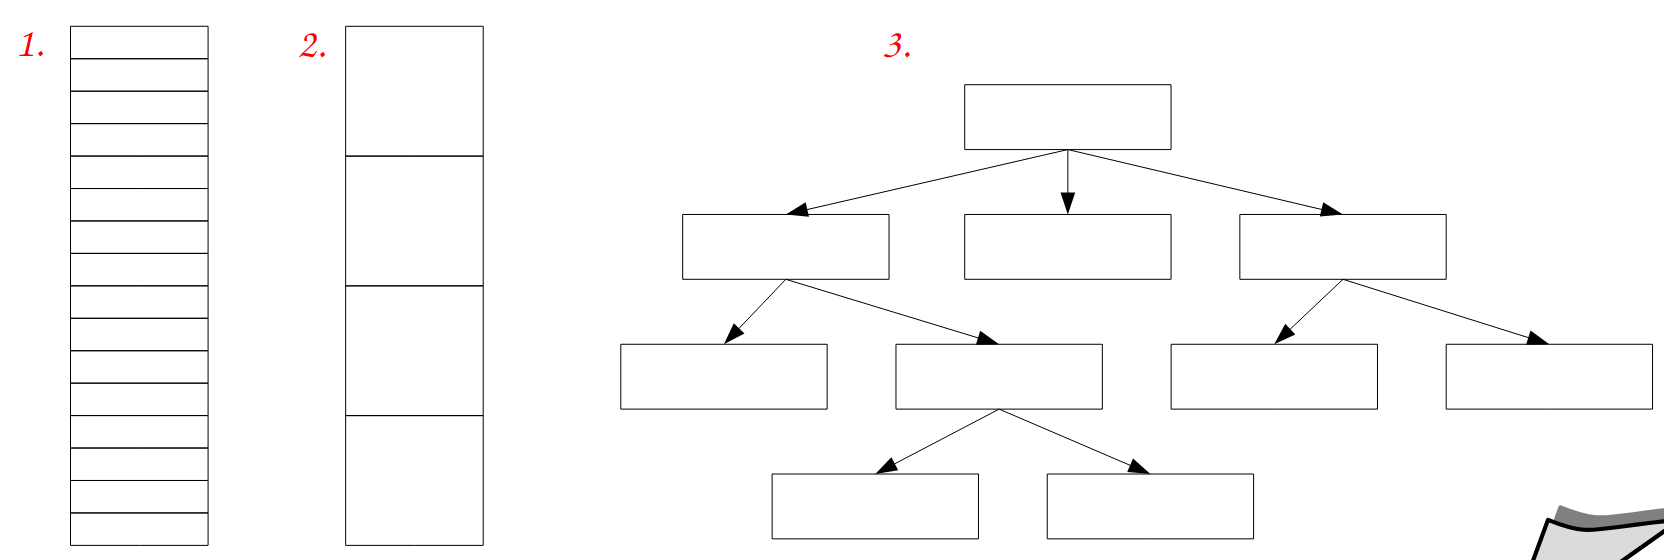
\includegraphics[width=0.7\linewidth]{Images/Screenshot 2025-01-18 at 15-45-24 so-07-filesystem.pdf.png}
\end{figure}

I sistemi operativi possono attuare diverse scelte nella
gestione della struttura dei file.

Scelta minimale: i file sono considerati semplici stringhe di byte, a parte i file eseguibili il cui formato è dettato dal s.o. .

Parte strutturata/parte a scelta dell'utente.

Diversi tipi di file predefiniti.

Dunque è un trade-off.
Più formati rendono il codice di sistema più ingombrante, causano incompatibilità di programmi (accesso a file di formato differente), ma permmettono una  gestione efficiente e non duplicata per i formati speciali.

Invece meno formati rendono il codice di sistema più snello.

\newpage
\subsubsection{Metodi di accesso}
\begin{itemize}
    \item Sequenziale: read, write
    \item Accesso diretto: read pos, write pos \textit{(oppure operazione seek)}.
    \item Indicizzato: read key, write key \textit{(tipico dei database)}.
    \item A indice: è una tabella di corrispondenza chiave-posizione. 
\end{itemize}

\subsubsection{Operazioni sui file}
Operazioni fondamentali sui file:
\begin{itemize}
    \item creazione
    \item apertura/chiusura
    \item lettura/scrittura/append
    \item posizionamento
    \item cancellazione
    \item troncamento
    \item lettura/scrittura attributi
\end{itemize}

L'API (interfaccia per la programmazione) relativa alle
operazioni su file è basata sulle operazioni open/close. 

I file devono essere “aperti” prima di effettuare operazioni e “chiusi” al termine.

L’astrazione relativa all’apertura/chiusura dei file è utile per
mantenere le strutture dati di accesso al file, controllare le modalità di accesso/gestire gli accessi concorrenti e definire un descrittore per le operazioni di accesso ai dati.
\newpage
\subsection{Directory}

L'organizzazione dei file system è basata sul concetto di directory, che fornisce un'astrazione per
un'insieme di file. 
In molti sistemi, le directory sono file speciali.

\subsubsection{Operazioni sulle directory}
Operazioni definite sulle directory:
\begin{itemize}
    \item creazione
    \item cancellazione
    \item apertura di una directory
    \item chiusura di una directory
    \item lettura di una directory
    \item rinominazione
    \item link/unlink    
\end{itemize}

\subsection{Strutture delle directory}

La struttura di una directory può essere: a livello singolo, a due livelli, ad albero, a grafo aciclico, a grafo.

\subsubsection{Directory strutturata ad albero}
\begin{figure} [h]
    \centering
    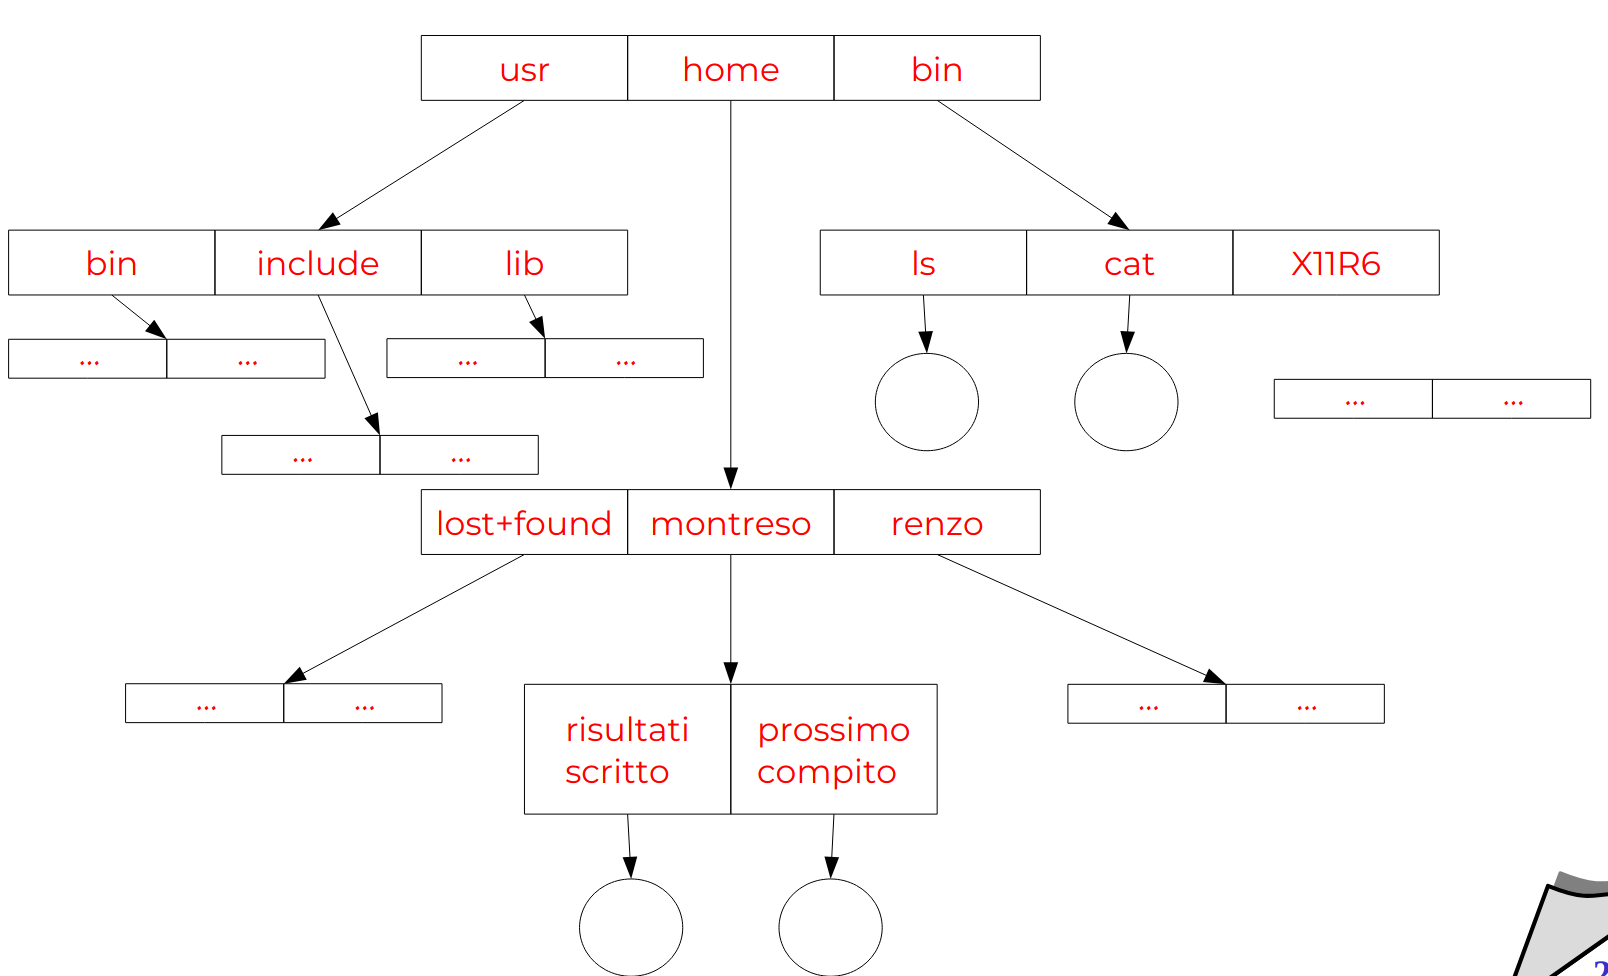
\includegraphics[width=0.7\linewidth]{Images/Screenshot 2025-01-18 at 16-02-00 so-07-filesystem.pdf.png}
\end{figure}

\subsubsection{Directory strutturate a grafo aciclico}
\begin{figure} [h]
    \centering
    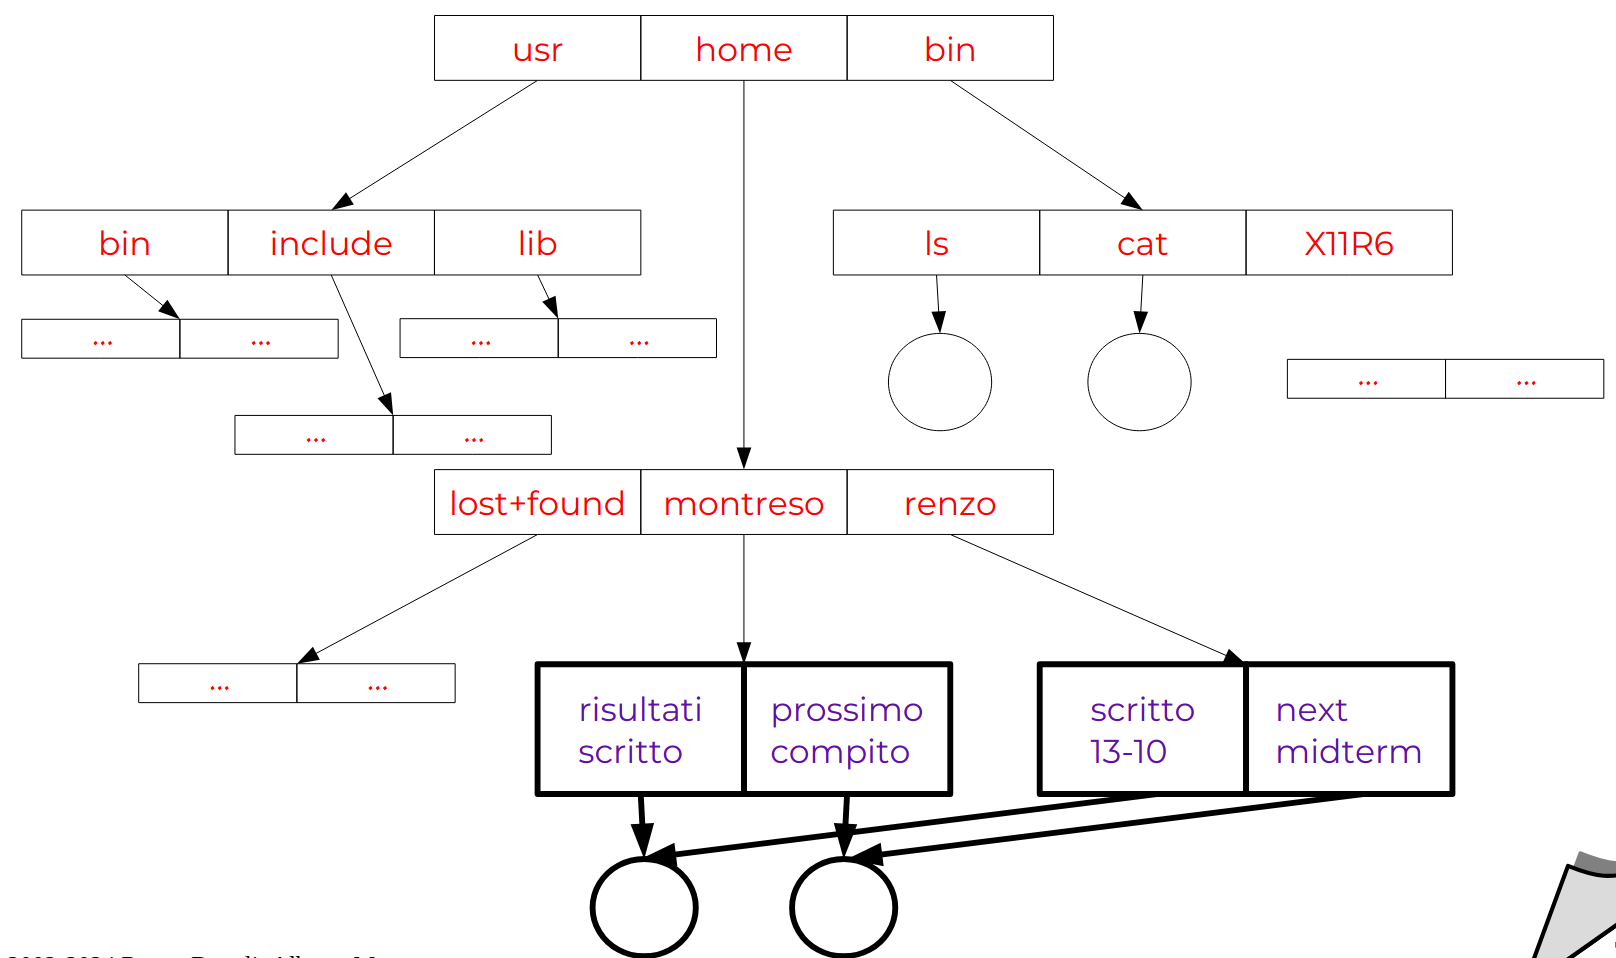
\includegraphics[width=0.7\linewidth]{Images/Screenshot 2025-01-18 at 16-04-34 so-07-filesystem.pdf.png}
\end{figure}

In un sistema operativo multitasking, i processi accedono ai
file indipendentemente.

\paragraph{Come vengono viste le modifiche ai file da parte dei vari processi?}
In UNIX, le modifiche al contenuto di un file aperto vengono rese visibili agli altri processi immediatamente. Esistono due tipi di condivisione del file: condivisione del puntatore alla posizione corrente nel file, oppure condivisione con distinti puntatori alla posizione corrente.


\section{Visione implementazione}


\paragraph{Implementazione del file system}

I problemi da tenere in considerazione: 
organizzazione di un disco, allocazione dello spazio in blocchi, gestione spazio libero, implementazione delle directory, tecniche per ottimizzare le prestazioni, tecniche per garantire la coerenza.

\subsection{Organizzazione del disco}
\paragraph{Struttura del disco:} un disco può essere diviso in una o più partizioni, porzioni indipendenti del disco che possono ospitare file system distinti.

Il primo settore dei dischi è il cosiddetto \textbf{master boot record} (MBR) è utilizzato per fare il boot del sistema.
Esso contiene la \textbf{partition table}, l'indicazione della partizione attiva e al boot, il MBR viene letto ed eseguito.
\begin{figure} [h]
    \centering
    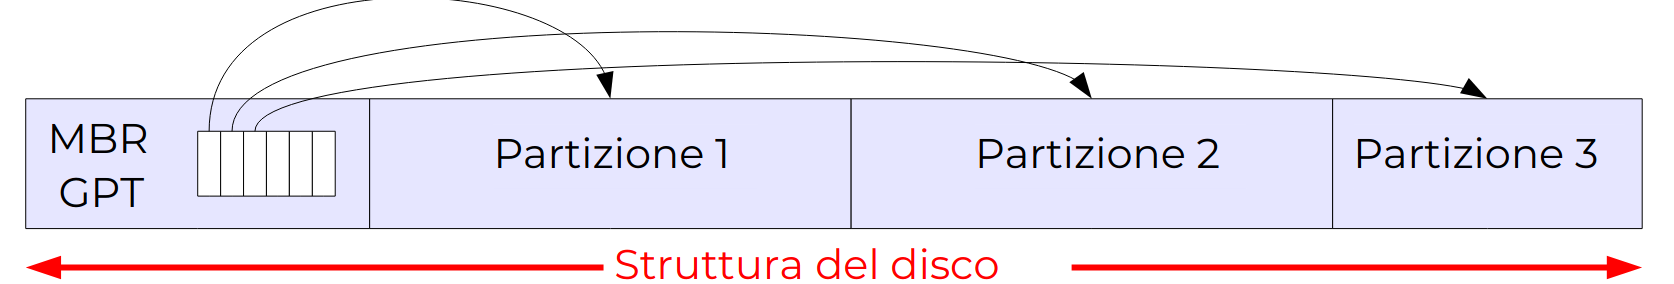
\includegraphics[width=0.7\linewidth]{Images/Screenshot 2025-01-18 at 16-10-24 so-07-filesystem.pdf.png}
\end{figure}

\paragraph{Struttura di una partizione}
Ogni partizione inizia con un boot block, il MBR carica il boot block della partizione attiva e lo esegue.

Il boot block carica il sistema operativo e lo esegue.

L'organizzazione del resto della partizione dipende dal file system.

\begin{figure} [h]
    \centering
    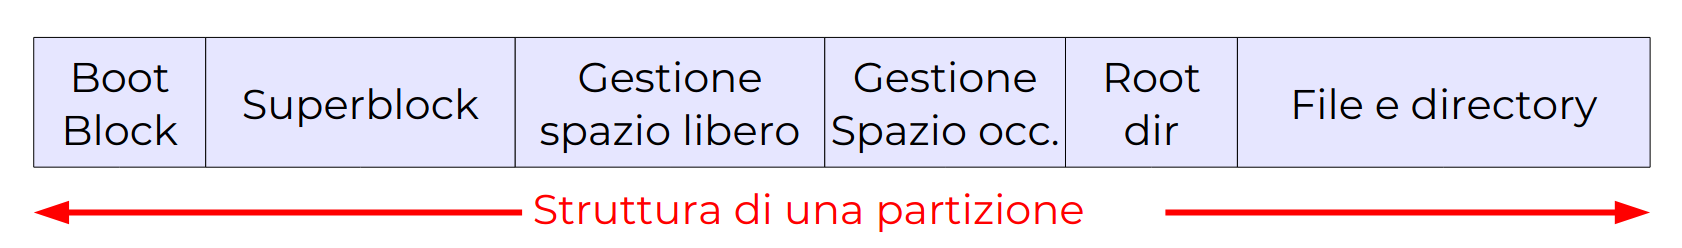
\includegraphics[width=0.7\linewidth]{Images/Screenshot 2025-01-18 at 16-12-24 so-07-filesystem.pdf.png}
\end{figure}

\newpage

\subsection{Allocazione}
L’hardware e il driver del disco forniscono accesso al disco visto
come un insieme di blocchi dati di dimensione fissa.

Come vengono scelti i blocchi dati da utilizzare per
un file e come questi blocchi dati vengono collegati assieme a
formare una struttura unica? 

Questo è il problema dell'allocazione.
\subsubsection{Allocazione contigua}
\paragraph{Descrizione:} i file sono memorizzati in sequenze
contigue di blocchi di dischi.
\paragraph{Vantaggi:} non è necessario utilizzare strutture dati per collegare i blocchi. 
L'accesso sequenziale è efficiente poichè i blocchi contigui non necessitano operazioni di seek.

L'accesso diretto è efficiente:
\newline
\textbf{block}= offset / blocksize
\newline
\textbf{pos}= offset $\%$ blocksize

\paragraph{Svantaggi:} si ripropongono tutte le problematiche dell’allocazione contigua in memoria centrale \textit{(frammentazione esterna, politica di scelta dell’area di blocchi liberi da usare per allocare spazio per un file)}.

Inoltre i file non possono crescere di dimensione.

\begin{figure} [h]
    \centering
    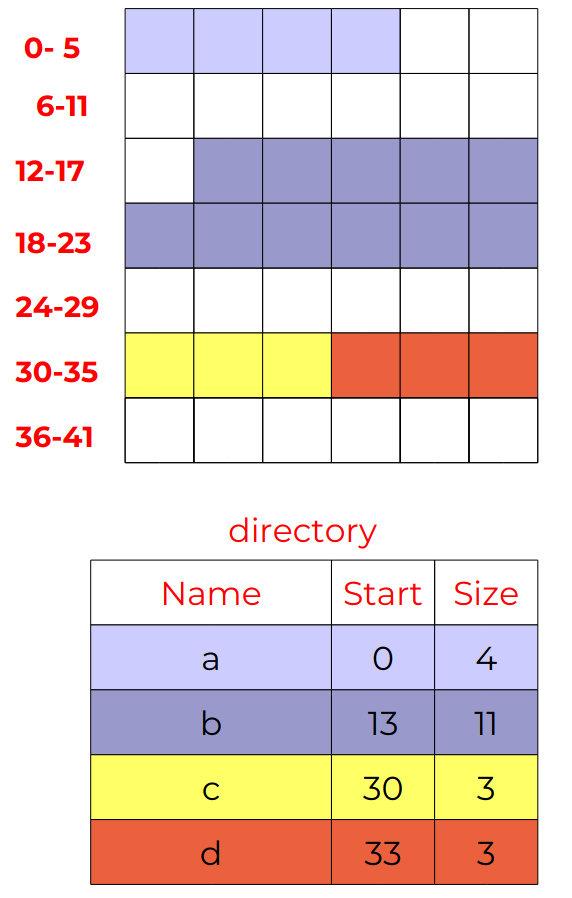
\includegraphics[width=0.3\linewidth]{Images/Screenshot 2025-01-18 at 16-21-15 so-07-filesystem.pdf.png}
\end{figure}

\subsubsection{Allocazione concatenata}
\paragraph{Descrizione:} ogni file è costituito da un lista concatenata di blocchi dove ogni blocco contiene un puntatore al blocco successivo. Il descrittore del file contiene i puntatori al primo e all’ultimo elemento della lista.

\paragraph{Vantaggi:} risolve il problema della frammentazione esterna. L’accesso sequenziale o in “append mode" è efficiente.
\paragraph{Svantaggi:} L’accesso diretto è inefficiente, progressivamente l’efficienza globale del file system degrada
\textit{(i blocchi sono disseminati nel disco, aumenta il n. di seek)}.

La dimensione utile di un blocco non è una potenza di due.
Se il blocco è piccolo (512 byte) l’overhead per i puntatori può essere rilevante.

\begin{figure} [h]
    \centering
    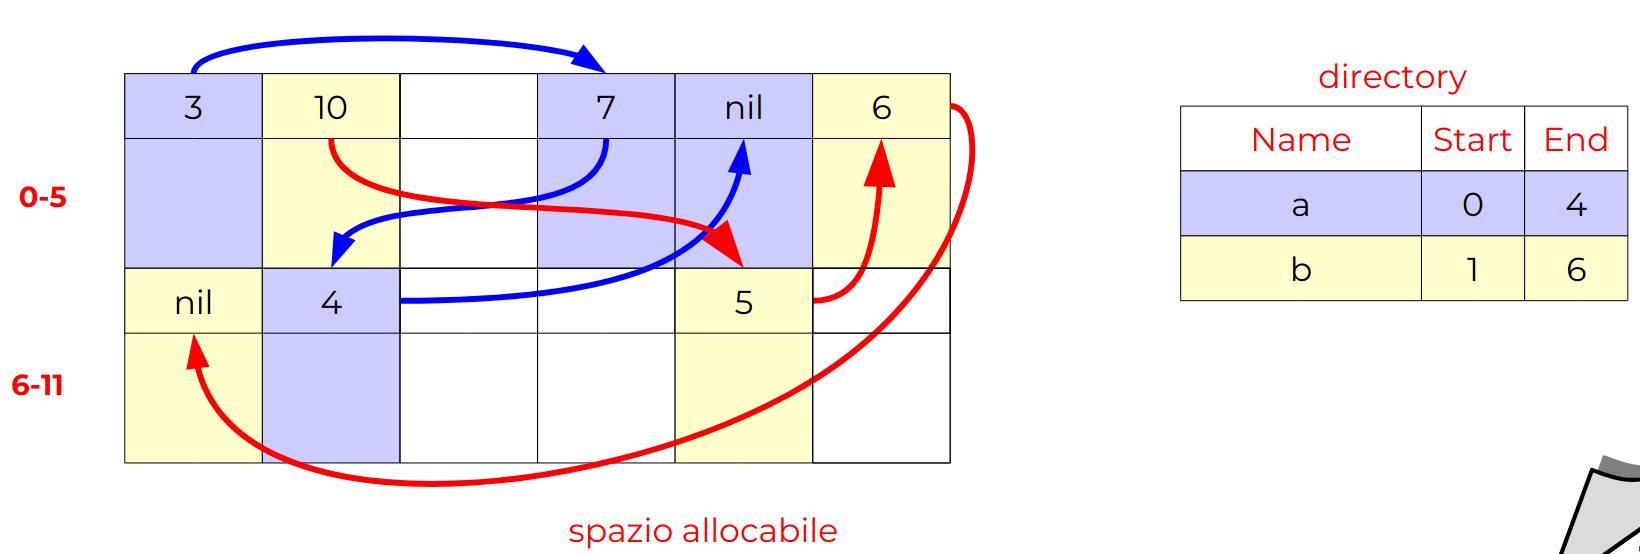
\includegraphics[width=0.7\linewidth]{Images/Screenshot 2025-01-18 at 16-26-12 so-07-filesystem.pdf.png}
\end{figure}
\newpage
\subsubsection{Allocazione basata su FAT}

\paragraph{Descrizione:} invece di utilizzare parte del blocco dati per contenere il puntatore al blocco successivo
si crea una tabella unica con un elemento per blocco (o per cluster).

\paragraph{Vantaggi:}i blocchi dati sono interamente dedicati ai dati, possibile fare caching in memoria dei blocchi FAT. 
L'accesso diretto diventa così più efficiente, in quanto la lista di puntatori può essere seguita in memoria.
\textit{(metodo usato da DOS, macchine fotografiche, chiavette
USB)}
\paragraph{Svantaggi} la scansione richiede anche la lettura della FAT, aumentando così il numero di accessi al disco.

\begin{figure} [h]
    \centering
    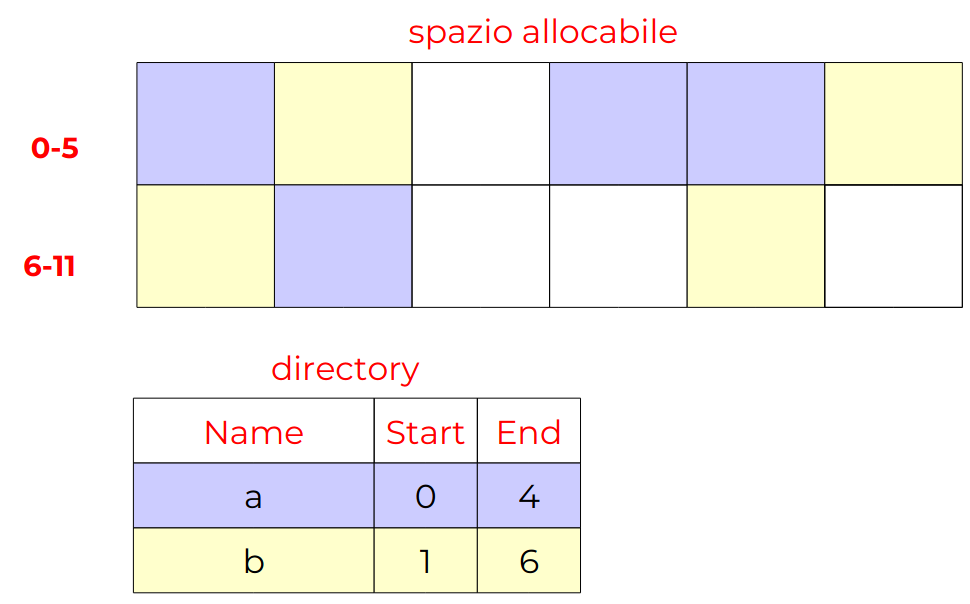
\includegraphics[width=0.4\linewidth]{Images/Screenshot 2025-01-18 at 16-35-55 so-07-filesystem.pdf.png}
\end{figure}

\begin{figure} [h]
    \centering
    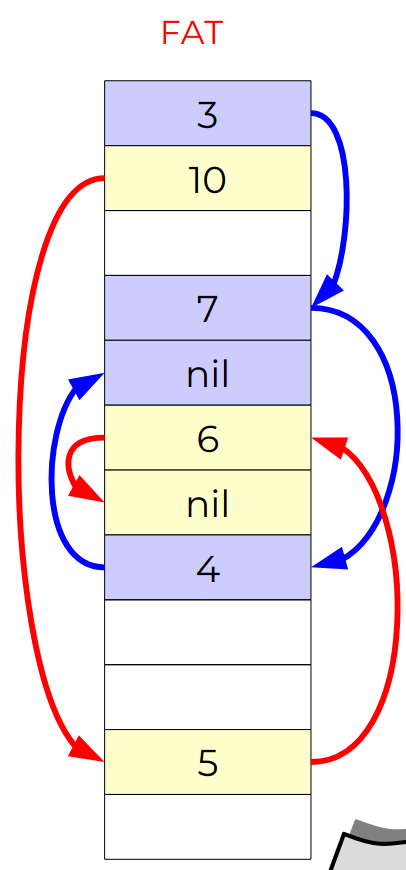
\includegraphics[width=0.17\linewidth]{Images/Screenshot 2025-01-18 at 16-36-06 so-07-filesystem.pdf.png}
\end{figure}

\subsubsection{Allocazione indicizzata}
\paragraph{Descrizione:} l'elenco dei blocchi che compongono un file viene memorizzato in un blocco indice.

Per accedere ad un file, si carica in memoria la sua area indice e si utilizzano i puntatori contenuti.

\paragraph{Vantaggi:} risolve il problema della
frammentazione esterna, è efficiente per l’accesso diretto, il blocco indice deve essere caricato in memoria solo quando il file
è aperto.

\paragraph{Svantaggi:} la dimensione del blocco indice determina l’ampiezza massima del file, utilizzare blocchi indici troppo grandi comporta un notevole spreco di spazio.

\paragraph{Come risolvere il trade-off?}

\begin{figure} [h]
    \centering
    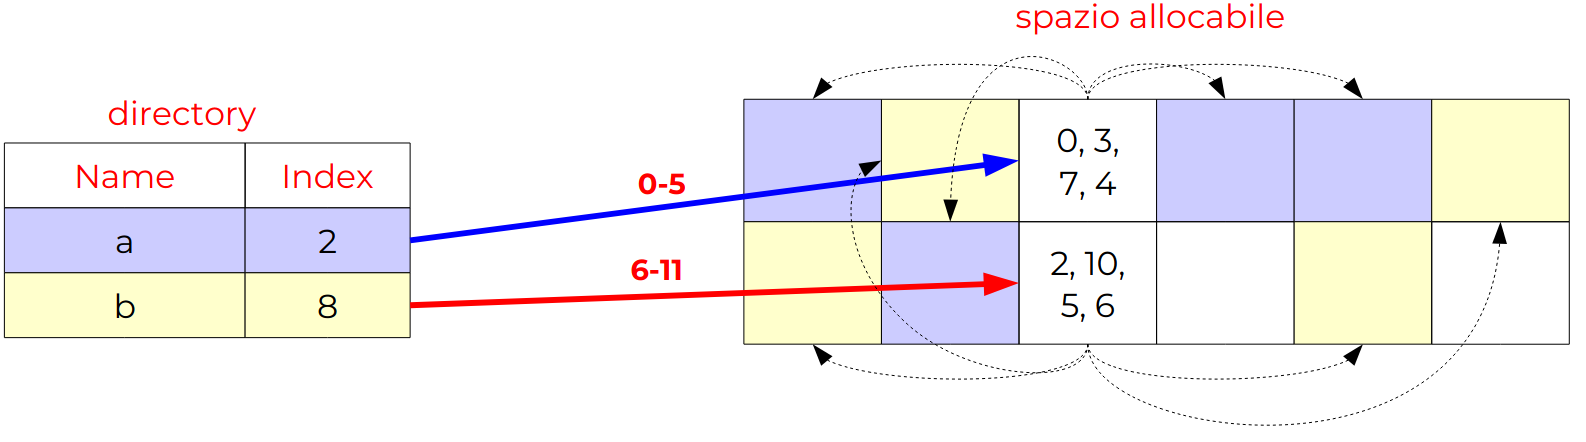
\includegraphics[width=0.7\linewidth]{Images/Screenshot 2025-01-18 at 16-40-54 so-07-filesystem.pdf.png}
\end{figure}



\subsubsection{Allocazione indicizzata - Possibili soluzioni}
\paragraph{Concatenazione di blocchi indice}
l’ultimo elemento del blocco indice non punta al blocco dati ma al
blocco indice successivo.
Si ripropone il problema per l’accesso diretto a file di grandi
dimensioni.
\begin{figure} [h]
    \centering
    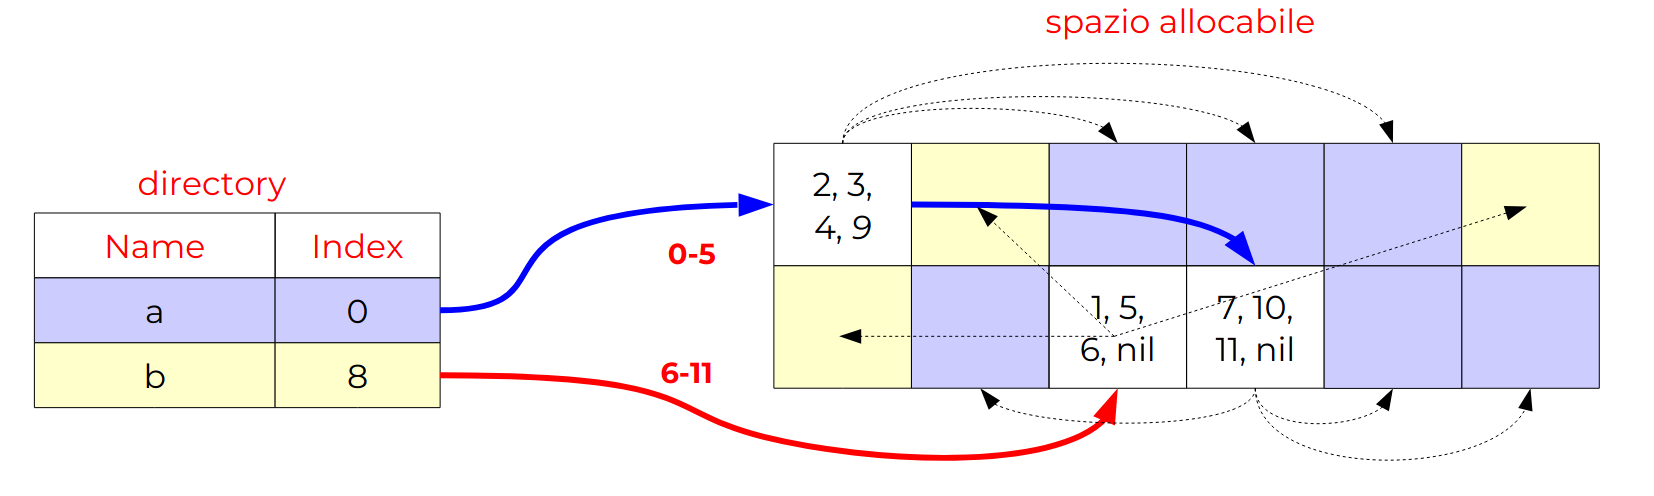
\includegraphics[width=0.7\linewidth]{Images/Screenshot 2025-01-18 at 16-47-32 so-07-filesystem.pdf.png}
\end{figure}

\paragraph{Indice multilivello}
si utilizza un blocco indice dei blocchi indice.
Degradano le prestazioni, in quanto richiede un maggior numero di
accessi.

\begin{figure} [h]
    \centering
    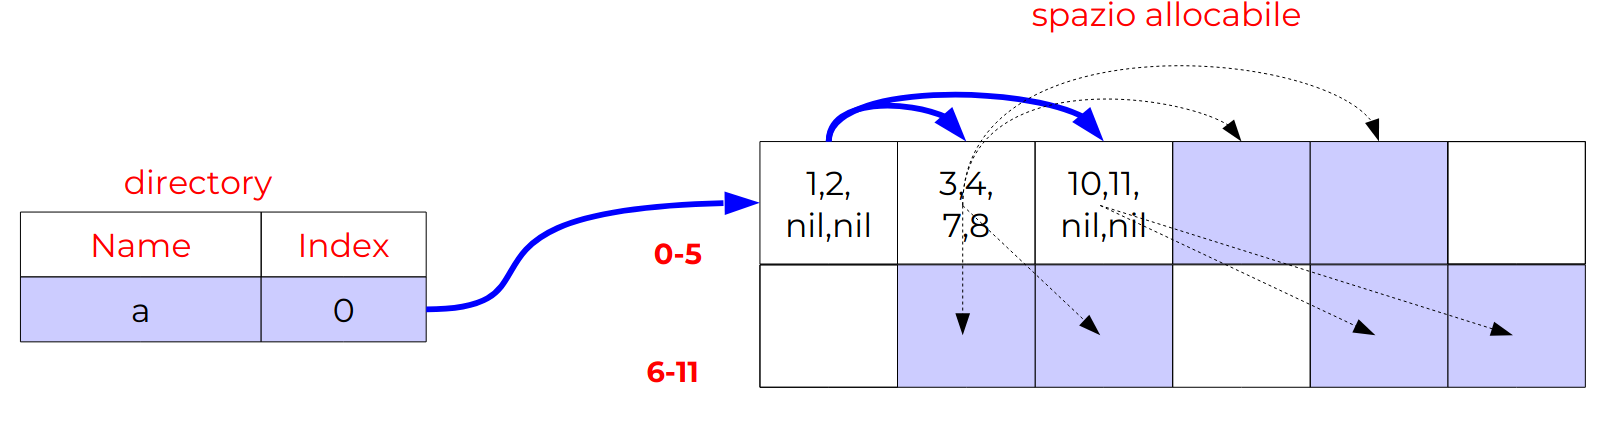
\includegraphics[width=0.7\linewidth]{Images/Screenshot 2025-01-18 at 16-45-53 so-07-filesystem.pdf.png}
\end{figure}

\subsubsection{Allocazione indicizzata e UNIX}

In UNIX ogni file è associato ad un \textbf{i-node} (index node).
Un i-node è una struttura dati contenente gli attributi del file, e un indice di blocchi diretti e indiretti, secondo uno schema misto.

\begin{figure} [h]
    \centering
    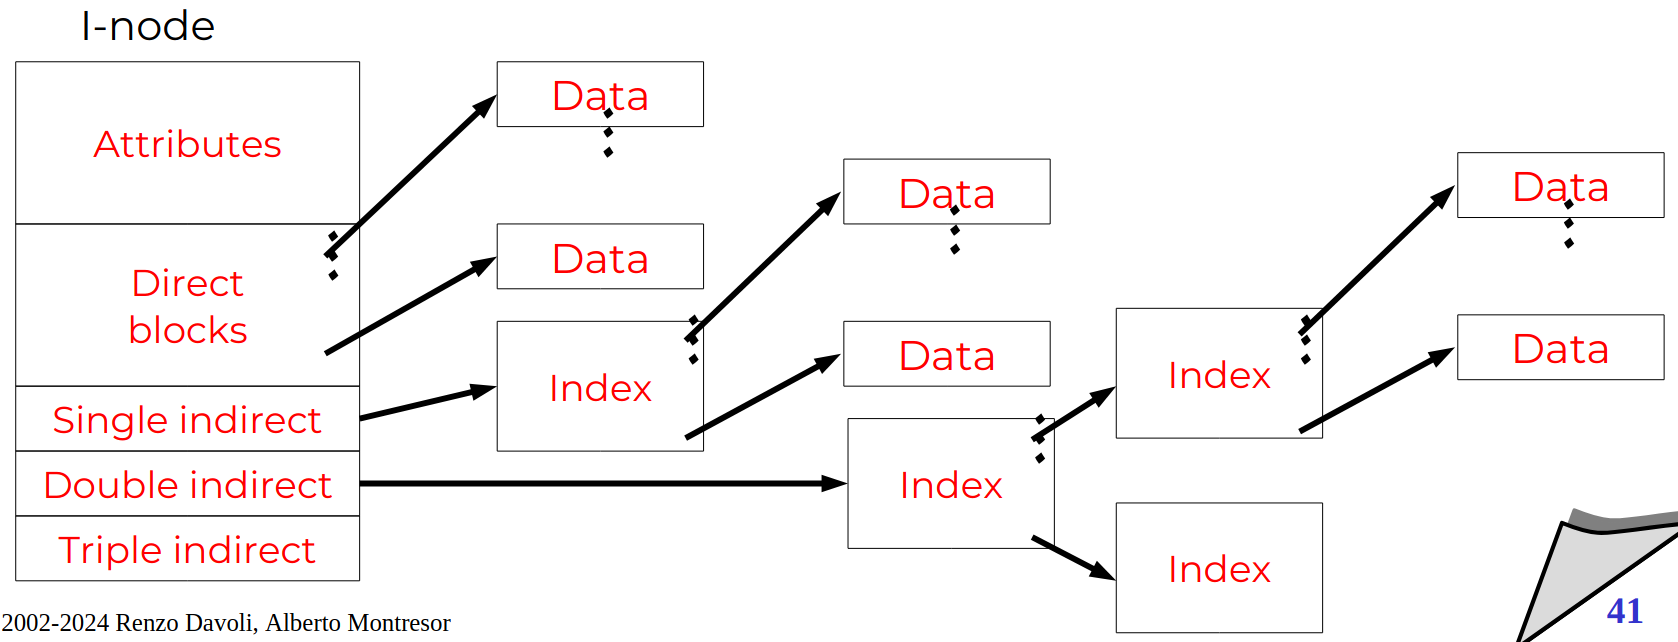
\includegraphics[width=0.7\linewidth]{Images/Screenshot 2025-01-18 at 16-49-53 so-07-filesystem.pdf.png}
\end{figure}

\paragraph{Allocazione e performance}
Lo schema UNIX garantisce buone performance nel caso di accesso sequenziale, file brevi sono acceduti più velocemente e occupano meno memoria.

Ci sono anche ulteriori miglioramenti, il pre-caricamento \textit{(per esempio nell’allocazione concatenata fornisce buone prestazioni per l’accesso sequenziale)}, combinazione dell’allocazione contigua e indicizzata, contigua per piccoli file ove possibile, indicizzata per grandi file.

\subsection{Gestione spazio libero}
\subsubsection{Mappa di bit}
\paragraph{Descrizione:} ad ogni blocco corrisponde un bit in una bitmap. I blocchi liberi sono associati ad un bit di valore 0, i blocchi occupati sono associati ad un bit di valore 1.
\paragraph{Vantaggi:} semplice, è possibile selezionare aree contigue.
\paragraph{Svantaggi:} la memorizzazione del vettore può richiedere molto spazio.
\begin{figure} [h]
    \centering
    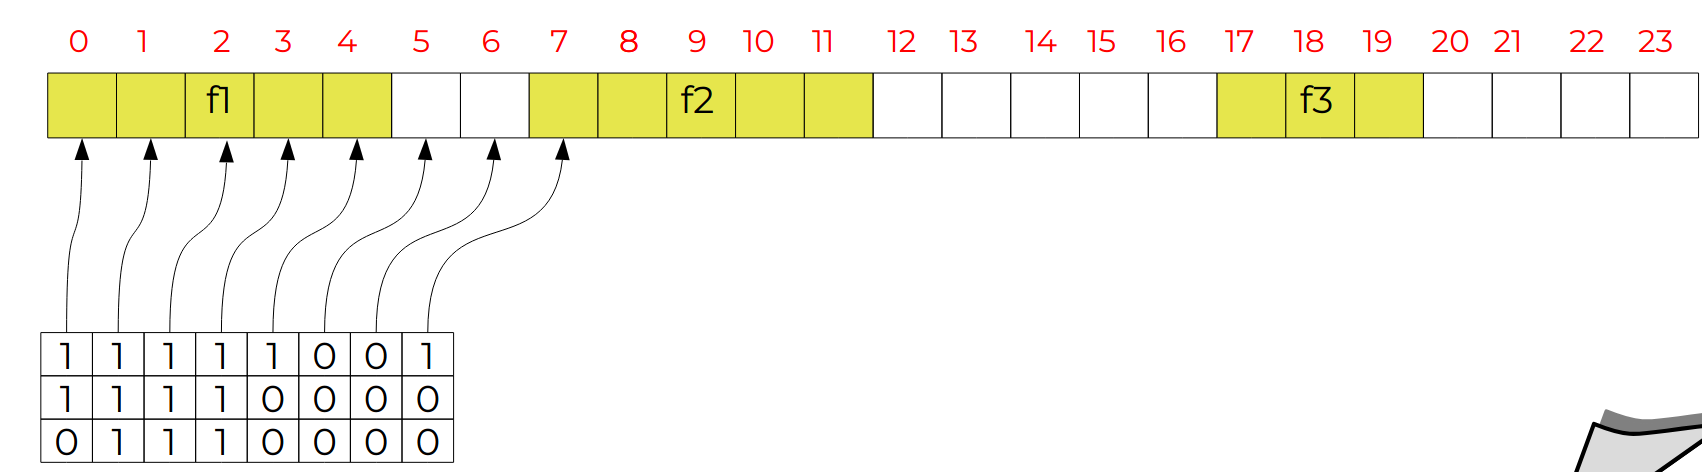
\includegraphics[width=0.8\linewidth]{Images/Screenshot 2025-01-18 at 16-55-04 so-07-filesystem.pdf.png}
\end{figure}
\newpage
\subsubsection{Lista concatenata}
\paragraph{Descrizione:} blocchi liberi vengono mantenuti in una lista concatenata, si integra perfettamente con il metodo FAT
per l'allocazione delle aree libere.

\paragraph{Vantaggi:} richiede poco spazio in memoria centrale.
\paragraph{Svantaggi:} l’allocazione di un’area di ampie dimensioni è costosa e l’allocazione di aree libere contigue è molto difficoltosa.
\begin{figure} [h]
    \centering
    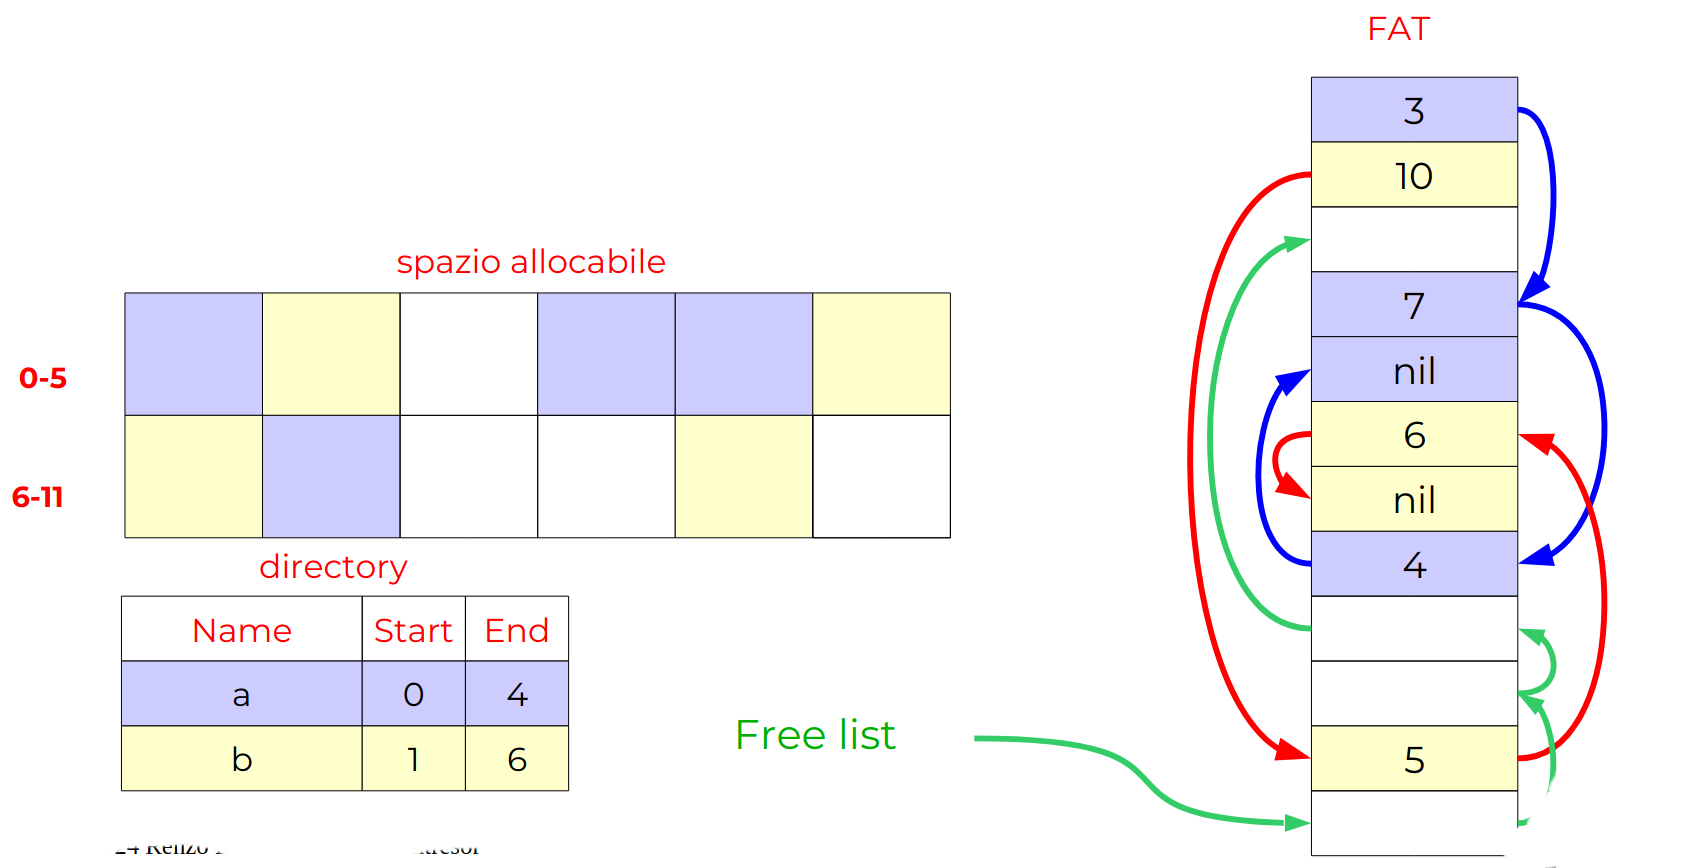
\includegraphics[width=0.7\linewidth]{Images/Screenshot 2025-01-18 at 17-00-54 so-07-filesystem.pdf.png}
\end{figure}

\subsubsection{Lista concatenata (blocchi)}

\paragraph{Descrizione:} è costituita da una lista concatenata di blocchi contenenti puntatori a blocchi liberi.

\paragraph{Vantaggi:} ad ogni istante, è sufficiente mantenere in memoria semplicemente un blocco contenente elementi liberi.
Non è necessario utilizzare una struttura a dati a parte; i blocchi contenenti elenchi di blocchi liberi possono essere
mantenuti all'interno dei blocchi liberi stessi.
\paragraph{Svantaggi:} l’allocazione di un’area di ampie dimensioni è costosa e l’allocazione di aree libere contigue è molto difficoltosa

\begin{figure} [h]
    \centering
    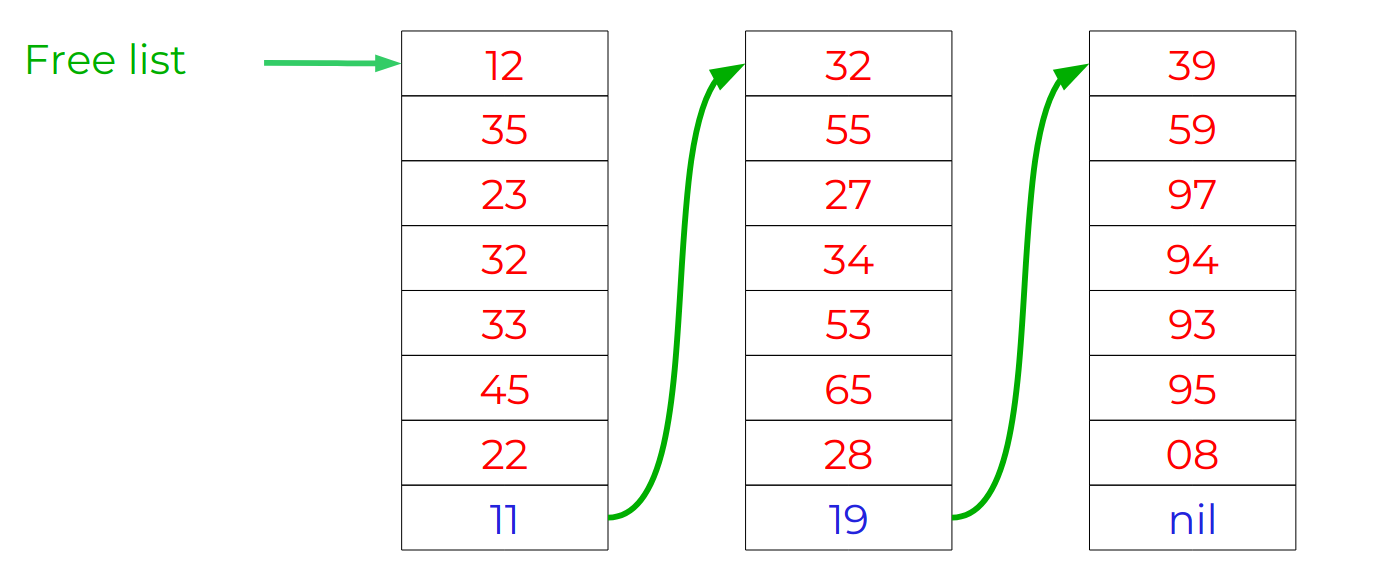
\includegraphics[width=0.7\linewidth]{Images/Screenshot 2025-01-18 at 17-02-36 so-07-filesystem.pdf.png}
\end{figure}

(fine slide 48)